\chapter{乡村旅游}
\label{chapter:travel}

\begin{figure}[htbp]
    \centering
    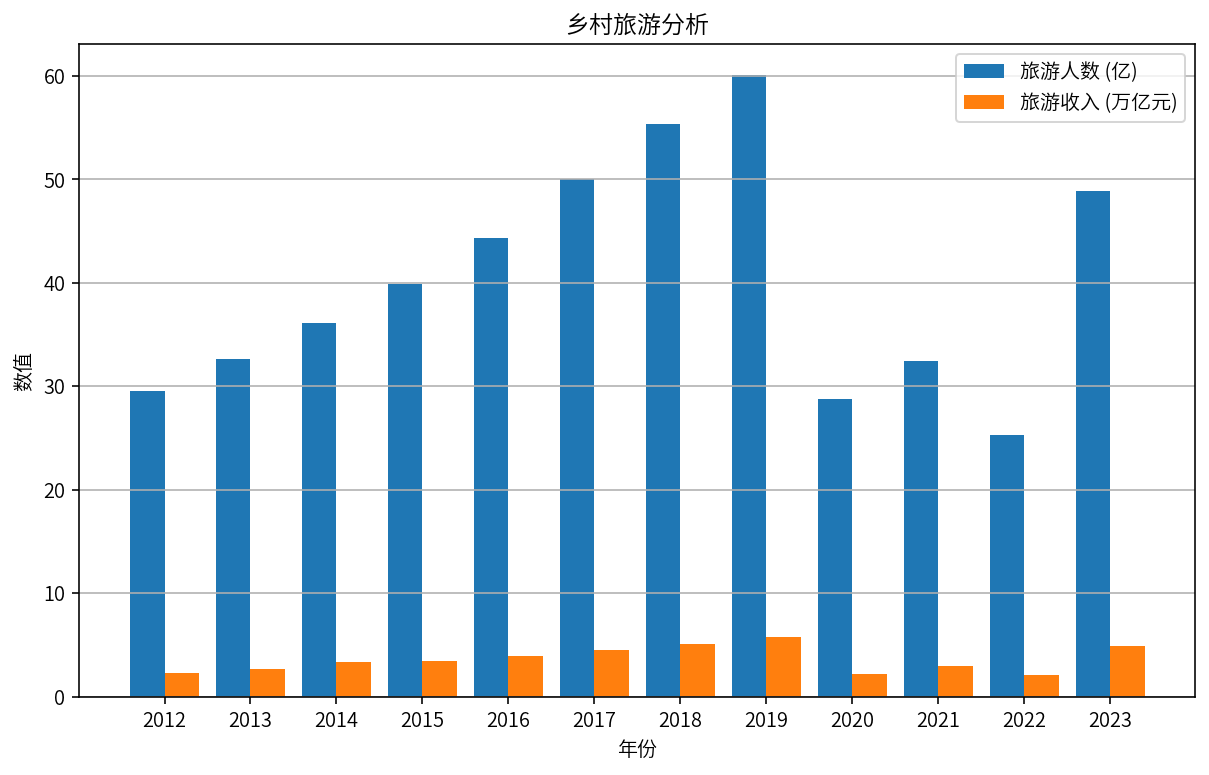
\includegraphics[width=0.5\linewidth]{figures/10.png}
    \caption{近十年乡村旅游人数与旅游收入}
\end{figure}

%GPT引导语:对于乡村旅游对乡村振兴的发展影响,我们分析了近十年去往乡村旅游的人数和旅游收入,发现前几年去往乡村旅游人数和旅游收入不断上涨,可能是因为城市的快节奏发展带来的压力使人们偏爱去往乡村旅游放松。但在2020年出现断崖式下跌,分析可能是因为受到新冠疫情防控的影响导致。在其之后疫情防控解除后又缓慢回升。目前经济开始复苏,旅游业也开始恢复生机。预计未来旅游业也会持续为乡村带来经济流动。

乡村旅游作为乡村振兴战略中的重要组成部分,近年来在促进农村经济多元化、农民增收以及城乡融合等方面发挥了显著作用。通过深入分析过去近十年来乡村旅游接待游客数量及其所带来的旅游总收入变化趋势,我们可以看到,在此期间,随着城市化进程的加快和生活节奏的不断提速,越来越多的城市居民开始向往乡村的宁静与自然环境,寻求从喧嚣中暂时解脱,回归田园以放松身心。这种趋势直接反映在逐年攀升的乡村旅游人数和收入上,显示出乡村旅游市场的蓬勃生机。

然而,在2020年,全球范围内的新冠疫情爆发对包括乡村旅游在内的整个旅游业造成了前所未有的冲击。为应对疫情扩散,各国政府采取了严格的防控措施,包括旅行限制、社交距离规定等,这些措施无疑对依赖人员流动性的乡村旅游产业带来了断崖式的影响,表现为接待游客数急剧减少,旅游收入大幅下滑。

随着时间推移,尤其是在疫情防控取得阶段性成果并逐步解除相关限制后,乡村旅游市场开始显现复苏迹象。各地政府及相关部门积极出台一系列扶持政策,推动乡村旅游产业升级转型,鼓励发展特色民宿、生态农业体验、地方文化活动等多种形式的乡村旅游产品,以适应后疫情时代消费者的新需求。同时,随着国内经济整体形势的好转和社会消费信心的恢复,去往乡村旅游的人次和旅游收入也呈现出缓慢回升的态势。

展望未来,预计在持续强化疫情防控常态化的前提下,旅游业特别是乡村旅游将会进一步融入乡村振兴的整体布局中,通过优化旅游资源、提升服务品质、创新旅游业态等方式,继续发挥其在拉动内需、激活乡村经济、带动农民就业等方面的积极作用,为乡村地区的经济发展注入持久动力。